\documentclass[12 pt]{article}
%\usepackage[utf8]{inputenc}
\usepackage{amsmath}
\usepackage{amssymb}
\usepackage{geometry}
\usepackage{fancyhdr}
\usepackage{setspace}
\usepackage{graphicx}
%\usepackage{lineno}
\usepackage[english]{babel}
\usepackage[round]{natbib}

\renewcommand\headrulewidth{0 pt}
\pagestyle{fancy}
\fancyhf{}
\rfoot{\thepage}

\setstretch{2}

\geometry{tmargin=2.5 cm, bmargin=3 cm, lmargin=3 cm, rmargin=3 cm}

%\bibliographystyle{JournalofAnimalEcology}
\bibliographystyle{besjournals}

\begin{document}

\begin{Large}
\noindent \textbf{Title:} Potential impacts of climate change on the phenological synchrony between a consumer and its resource: the example of the spruce budworm and its tree host 
\end{Large}
\vspace{1 cm}

\noindent \textbf{Authors:} Portalier S.M.J.$^{1}$, Candau J.N.$^2$, Lutscher F.$^1$ \\
\textbf{Institutions:} \\
$^1$: Department of Mathematics and Statistics, university of Ottawa, Ottawa, ON, Canada \\
$^2$: Natural Resources Canada, Canadian Forest Service, Great Lakes Forestry Centre, Sault Ste Marie, ON, Canada\\
%\textbf{Corresponding author:} \\
%name: S\'ebastien Portalier \\
%address: Department of Mathematics and Statistics, university of Ottawa, STEM Complex, 150 Louis-Pasteur Pvt, K1N 6N5, Ottawa, ON, Canada \\
%email: sportali@uottawa.ca \\

%\clearpage

\section*{Abstract}
The ongoing anthropogenic climate change increasingly affects species phenology. Especially, the seasonal resting period, when organisms remain inactive during part of the year, is often driven by temperature. In the case of a consumer and a resource that both exhibit a seasonal resting period, the synchrony of the end of their respective resting period is fundamental for the persistence of their interaction. Since the consumer and its resource may react differently to a change in temperature regime, the synchrony between them will likely be altered. In this study, we propose a general theoretical model that determines the duration of the resting period according to temperature, and its effects on synchrony or mismatch between phenological stages of two interacting species. We then illustrate our approach using the spruce budworm – balsam fir system in Eastern Canada as a case study. We found that an increase in temperature would usually advance the end of the resting period. However, the effects of a warm or cold spell during the resting period would strongly vary according to the time and the duration of the spell. Depending on the way each species reacts to the same temperature shift, the mismatch between the consumer and its resource may increase or decrease. For the spruce budworm – balsam fir system, our model predicts that an increase in temperature may increase the mismatch between the insect and the tree in Southern sites, but may increase the synchrony in Northern sites. This kind of modelling approach is of primer importance to investigate potential effects of climate change on consumer – resource systems. The study of synchrony between interacting species is fundamental to predict future species distribution.\par

\noindent \textbf{Keywords:} Consumer, resource, phenology, global warming, spruce budworm, balsam fir

\clearpage

\section{Introduction}
Anthropogenic climate change has increasingly disrupted ecological interactions for the past century (IPCC 2014 and references within). It is expected that this trend will continue and amplify as interacting species are likely to respond differently to similar environmental changes and selective pressures \citep{Parmesan2006}. Among ecological interactions, consumer-resource relationships are fundamental to the functioning of terrestrial and marine ecosystems. Trophic interactions between consumers and resources may be affected by climate change through: (1) direct changes in the life history traits (e.g., fecundity, mortality) of the consumer and/or the resource, (2) changes in the abundance of the consumer and/or the resource due to cascading effects from higher or lower trophic levels (e.g., changes in the consumer’s predators or competitors) \citep{Both2009}, and (3) differential shifts in the phenology of the consumer and/or the resource leading to phenological mismatch \citep{Kharouba2018}.\par
Phenological mismatch between a consumer and a resource occurs when the timing of the species' life cycle phases relevant to the interaction changes at different rates. The impact of a phenological mismatch on interacting species depends on the nature of the interaction and the direction of the phenological change \citep{Renner2018}. In antagonistic interactions such as between a consumer and a resource, an increase in synchrony will likely favour the consumer while a decrease will favour the resource. \par
While there is a growing body of literature stating evidence for changes in species phenology, examples of phenological mismatch are still relatively scarce \citep{Renner2018} partly because they are expecting to persist only for a short period of time over small spatial scales. Among studies, there is no clear pattern in the direction of the change because some interacting species are getting closer, while others are getting further apart \citep{Kharouba2018}. The clearest cases of climate-driven mismatch have been reported at high latitudes where many organisms rely on a seasonal resting period because temperatures affecting physiological processes tend to be below species optima for most of the year. After a seasonal arrest in development that can last for several months, synchrony in springtime phenology, particularly between the emergence of phytophagous insects from diapause and the end of their host plants dormancy, is critical to the consumer’s fitness \citep{VanAsch2007}. Spring defoliators have evolved to exploit foliage at its annual optima nutritional qualities, i.e., high concentration in nutrient and water and low concentrations in fibre and secondary metabolites \citep{Hunter1992,Mattson1987}. This strategy requires a precise phenological match between the consumer and its resource because the quality of foliage declines quickly with foliar expansion. If the consumer emerges too early, it may encounter a long initial period with no food or poor food quality. If it emerges too late, the speed at which the nutritional quality of the foliage degrades may outpace its capacity to adjust physiologically thus negatively impacting its fitness. \par   
The seasonal resting phase of many organisms can be divided in two successive stages called endodormancy and ecodormancy in perennial woody plants, and diapause and quiescence in insects \citep{Chuine2017}. Development and metabolism are generally inhibited by internal factors (e.g., depletion of energy reserves, hormones) in the first stage and by external factors (e.g., temperature, photoperiod) in the second one. This study focuses on a system where both a consumer and its resource show a seasonal resting period during part of the year (e.g., during winter). For both, we assume that the first stage of the seasonal resting period is accomplished early in the winter before the return of favourable conditions, a common case in temperate and colder climates, and that temperature is the main driver that triggers the end of the second stage and therefore the resting period. In the remainder of this paper, the expression "resting period" will imply the second stage of the seasonal resting period.\par 
Observed patterns of change in phenological synchrony as a result of climate change have been difficult to explain mechanistically. The aim of this study is to investigate potential effects of global warming on the phenological synchrony between a consumer and its resource in the likely case where each species reacts independently of one another to temperatures. We begin with the general theoretical aspects that determine the duration of the resting period according to temperature, and its effects on synchrony / mismatch between phenological stages of the two species. Then, we use a major insect pest of the Canadian boreal forest, the spruce budworm, and its main host, balsam fir, as a case study. We investigate the phenological mismatch across a gradient of latitudes, and the way this synchrony / mismatch is expected to vary with climate change in the future.\par

\section{Methods}
We begin with a unified description of the mechanism that determines the duration of the resting period of a consumer and its resource in terms of accumulation of ambient temperature. Then we list our data sources and explain the fitting methods for the spruce budworm / balsam fir system.  

\subsection{Theoretical development}
Throughout the resting period, an organism accumulates units of some quantity. The instantaneous rate of accumulation depends on the ambient temperature, and the resting period ends when a certain level of that quantity has been accumulated. For trees, this quantity can be heat, for example in degree-day models \citep{Colombo1998} or more recent nonlinear models \citep{Chuine2000,Desbiens2007}. For insects, the quantity can be the proportion of the corresponding life-cycle stage that they have completed \citep{Cobbold2011,Regniere2012}. Since the development rate is also temperature dependent, this quantity is ultimately also a measure of accumulated heat. \par 
We denote time by $t$ in days and temperature by $x = x(t)$ in degrees Celsius. The instantaneous rate of accumulation is some nonnegative function of temperature, denoted by $R = R(x)$. For the range of temperatures that occur during the resting phase, $R(x)$ is an increasing function. Indeed, while developmental rates typically decrease when temperatures exceed an upper threshold \citep{Deutsch2008,Amarasekare2014}, such temperatures do not generally arise during the resting phase. The resting period begins at some time $t_0$ and ends at such time t* when the accumulated quantity reaches a certain threshold level $F$. As noted by \cite{Chuine2017}, this concept of an accumulating quantity is "still the most important assumption in plant and animal phenology modelling". The fundamental equation that connects all these quantities and determines the end of the resting period is
\stepcounter{equation}
\begin{equation} \label{mainmodel}
    \int _{t_0} ^{t^*} R(x(t)) \mathrm{d}t = F. \tag{Eq. \theequation}
\end{equation}
A typical example for the accumulation rate function is the sigmoidal function
\stepcounter{equation}
\begin{equation} \label{sigmoidal}
    R(x)=\frac{1}{1+exp(b(x-c))}, \tag{Eq. \theequation}
\end{equation}
where $b < 0$ and $c$ are two parameters to be estimated from data \citep{Chuine2000,Rebaudo2018}. When the quantity of interest is the proportion of the life-cycle completed, it is natural to set the threshold level to be $F = 1$. If we divide \ref{mainmodel} by $F$ and include the term $1/F$ into the function $R$ in \ref{sigmoidal}, we can standardize notation and compare different rate functions. We illustrate the rate function in \ref{sigmoidal} as well as the condition in \ref{mainmodel} for two different species and two simplistic temperature time series in Fig. \ref{fig:generaltheory}. As temperature patterns during the resting period change because of global warming, the end time of the resting period of a species may shift. In particular, when temperatures increase, accumulation occurs faster and the end time is earlier (bottom right plot in Fig. \ref{fig:generaltheory}). \par
Two species, such as a consumer and its resource, will likely have different forms of the rate accumulation function $R$ or the same form with different combinations of parameters (e.g., $b$, $c$, and $F$) even in the same temperature regime (compare solid and dashed curves in Fig. \ref{fig:generaltheory}, bottom left panel), which typically leads to different end times of the resting period (bottom right panel). We denote these by $t_e ^*$ (emergence time) for the insect (consumer) and by $t_b ^*$ (budburst time) for the host trees (resource). We call the difference in end times the mismatch between the two species (i.e., $mismatch=t_e ^*-t_b ^*$). When the end times of the resting period of two species respond differently to climate change, then the mismatch between the two species will change. This is the fundamental quantity that we are interested in here. \par
This quantity is illustrated in the bottom right plot of Fig. \ref{fig:generaltheory}. One would expect that a consumer that crucially relies on a certain resource would have evolved a relatively small mismatch with that resource. However, this does not mean that its accumulation rate curve has to be the same as that of its resource. Even if the functional form is the same, many different parameter combinations in $R(x)$ in \ref{sigmoidal} lead to the same end time of the resting period. Hence, the mismatch might increase or decrease with changing temperature patterns. We use this theoretical model to predict general patterns of climate change-induced shifts in species end times and changes in the mismatch between interacting species. We use the spruce budworm and balsam fir system in eastern Canada to illustrate how estimated rate accumulation functions can be applied to different temperature scenarios to investigate how climate change may affect the phenological between these two species.

\subsection{The spruce budworm – balsam fir system} 

\subsubsection{Study system} 
The spruce budworm (SBW) (\textit{Choristoneura fumiferana}) is the most destructive insect defoliator of the North American boreal forests \citep{Fleming2000}. It feeds primarily on balsam fir (\textit{Abies balsamea}), white spruce (\textit{Picea glauca}), red spruce (\textit{Picea rubens}), and black spruce (\textit{Picea mariana}). This insect has a 1-year life cycle with a winter diapause at the second larval stage. The first stage of the diapause ends in late winter and is followed by a period of quiescence during which development resumes at a rate dependent on outside temperatures. Once this post-diapause development is completed, second instar larvae emerge from their hibernacula (cocoon-like structure) in late April to late May in Eastern Canada and Northeastern USA.\par 
After emergence, young larvae mine 1-year old needles until budburst. The larvae will start feeding on expanding buds and developing needles as soon as they become available. Year-old needles are nutrient poor \citep{Mattson1987}. In contrast, expanding needles from swelling buds have the maximum concentration of nitrogen and mineral elements thus providing nutrient-rich food to the developing larva. Hence, the success of SBW populations in establishing feeding sites in the spring depends on the synchrony of their development with that of their host trees \citep{Regniere2008,Volney2007}. Indeed, the population consequences for late-emerging SBW are severe: larval survival is depressed (from about $60\%$ normal survival down to $10\%$); development is delayed, and average pupal mass decreases by about $50\%$ for both sexes \citep{Lawrence1997}. In the boreal forests of Eastern Canada, the higher vulnerability of balsam fir to spruce budworm defoliation compared to other host species has been attributed to its early budburst phenology \citep{Blais1957}. Indeed, under similar environmental conditions, balsam fir's budburst occurs two weeks prior to black spruce, closer to spruce budworm emergence. Many environmental factors may affect budburst phenology including the accumulation of cold temperature during the dormancy (i.e., chilling temperatures), warm temperatures during the quiescent phase (i.e., forcing temperatures), photoperiod, or snowmelt. Balsam fir budburst phenology appears to be related to forcing temperatures but not photoperiod \citep{Osawa1983}. In Eastern Canada and Northeastern USA, emergence of SBW second instar larvae from their hibernacula generally precedes balsam fir budburst by several days.\par 
We present accumulation rate functions for spruce budworm and balsam fir separately. 

\subsubsection{Phenological model of spruce budworm's spring emergence}

Spruce budworm spends several months in its seasonal resting period. The factors involved in the termination of the first phase are unknown. For modelling purposes, the second stage of the seasonal resting period is often assumed to start on March 1st every year. and the  heat accumulation rate in this stage is defined as follows \citep{Regniere2012} 

\stepcounter{equation}
\begin{equation}\label{budworm}
    R(x(t)) = \left \lbrace
    \begin{array}{ll}
        \beta _1 \left[ \frac{1}{1+exp(\beta _2 + \beta _3 ^\tau)} -exp((\tau -1)/\beta _4) \right], & \text{if} \; x_b \leq x(t) \leq x_m \\
        0, & \text{otherwise}
    \end{array} \right . \tag{Eq. \theequation}
\end{equation} 
where
\stepcounter{equation}
\begin{equation}
    \tau = \frac{x(t)-x_b}{x_m - x_b} \tag{Eq. \theequation}
\end{equation}
Accumulation happens only when the temperature lies between a minimal value ($x_b$) and a maximal value ($x_m$). The resulting instantaneous rate of accumulation according to temperature shows a humped-shape profile. Accumulation is integrated through time (see Eq. 1), until $F = 1$. Parameter values for spruce budworm have been estimated from laboratory experiments as $\beta _1=0.194$,  $\beta _2=3.0$, $\beta _3=5.94$, $\beta _4=0.034$, $x_b = 2.5 \; ^{\circ}\text{C}$, and $x_m = 35 \; ^{\circ}\text{C}$ \citep{Regniere2012}.

\subsubsection{Phenological model of Balsam fir's budburst}

We use the Uniforc model of \citep{Chuine2000}, to model balsam fir's budburst phenology. Accordingly, the heat accumulation rate is the same as in the theoretical example (see \ref{sigmoidal}).\par
%\stepcounter{equation}
%\begin{equation}\label{balsam}
%    R(x(t))=\frac{1}{1+\exp (b_f(x(t)-c_f))}. \tag{Eq. \theequation}
%\end{equation}
Accumulation starts at a given time $t_0$, which is posterior to January 1st \citep{Desbiens2007}, when trees have accumulated enough cold to end bud dormancy. Accumulation is integrated through time (see \ref{mainmodel}). Budburst occurs when accumulation reaches a threshold $F^*$.\par
Fitting the model to data from Quebec and New Brunswick \citep{Desbiens2007} resulted in the following parameter values $b  = -0.1936$, $c = 10.99 \; ^{\circ}\text{C}$, $t_0 = 84$ (March 25th), and $F^*  = 13.63$, which differ only slightly from the parameterization by \cite{Desbiens2007}.\par
We perform sensitivity analysis on both models using partial rank correlation coefficient \citep{Wu2013}. 

\subsection{Temperature data}
We collected temperature data over a gradient of latitude in Eastern Canada (Fig. \ref{fig:map}) using BioSIM \citep{Regniere2014}. We used data from 1996 to 2016 to explore the latitudinal trends of emergence for the insect, budburst for the tree, and the mismatch between the two events over latitude and across years. \par
Last, we used predicted temperatures under different warming scenarios at the same locations in order to gain insights in expected trends for emergence, budburst and mismatch in the future. Selected scenarios are RCP2.6, RCP4.5 and RCP8.5 \citep{Vuuren2011}. \par
Both models used temperature data with a four-hourly time interval. It allows for the capture of warm events within a day (i.e., a few hours of warm temperatures, while the average daily temperature stays low). 

\section{Results}
\subsection{Theoretical results}
Model equation \ref{mainmodel} can in general not be solved explicitly for the end time, $t^*$, at least not for reasonable temperature time series $x(t)$. Instead, we consider how $t^*$ changes when a future temperature ($x_2(t)$) time series deviates from historical expectation ($x_1(t)$) by a small amount. We derive a general  approximation formula for the difference in the end times with regards to the two time series (see appendix). Here, we evaluate and discuss this formula for two particular cases: a constant temperature difference throughout the resting period or a warm or cold spell during a short time period. \par 

\subsubsection{Phenology shift of a single species}
In the case of a constant temperature difference, we write $x_2(t) = x_1(t)+\Delta x$ where $\Delta x$ is the difference. Then the corresponding end times t2* and t1* are then related by
\stepcounter{equation}
\begin{equation}\label{constant}
    t_2 ^* = t_1 ^* - \frac{\Delta x}{R(x_1(t_1 ^*))} \int _{t_0} ^{t_1 ^*} R'(x_1(t)) \mathrm{d}t \tag{Eq. \theequation}
\end{equation}
In the second case, if the difference in temperature between two years is a warm or cold spell of short duration $\Delta t$ at time $t_s$ of temperature difference $\Delta x$ (positive for a warm spell, negative for a cold spell), then the corresponding ends of the seasonal resting phases are related by
\stepcounter{equation}
\begin{equation}\label{spell}
    t_2 ^* = t_1 ^* - \Delta x \Delta t \frac{R'(x_1 (t_s))}{R(x_1(t_1 ^*))} \tag{Eq. \theequation}
\end{equation}
Both formulas show the expected qualitative pattern that if time series $x_2$ is warmer than $x_1$, i.e., $\Delta x >0$, then the phenology advances, i.e., end of the seasonal resting period $t_2 ^*$ is before the corresponding $t_1 ^*$ (since all the terms after the "$-$" sign are positive). More importantly, the formulas allow us to quantify the expected shift of the end time of the resting period. We observe that the shift depends on the derivative of the rate accumulation function. In particular, the impact of a short temperature spell is proportional to the derivative, $R'(x(t_s))$, at the time of the spell ($t_s$). Hence, the end time of the seasonal resting period is the most sensitive to warm or cold spells where $R(\cdot)$ has its maximal slope. For the rate function in \ref{sigmoidal}, this occurs at temperature $x=c$.

\subsubsection{Effects on the mismatch between two species}
Since there is no interaction during the resting phase, heat accumulation occurs independently in each species. For each species, we apply the formulas (\ref{constant} and \ref{spell}) for how the end times of the respective resting periods change when the temperature varies and then evaluate how the mismatch between the two species evolves. We denote the end times of the consumer for time series $x_i(t)$ by $t_{e,i}^*$ (emergence time) and of the resource by $t½{b,i}^*$ (budburst time). For our theoretical explorations, we choose a simplified temperature time series of daily mean temperatures. Specifically, we choose the cosine function
\stepcounter{equation}
\begin{equation}
    x_1(t) = 6.9 + 15 \cos\left(\frac{2\pi (t-200)}{365}\right), \tag{Eq. \theequation}
\end{equation}
where the mean, amplitude and offset have been chosen to match historical averages in the city of Fredericton (NB, Canada). We use the heat accumulation functions $R_b(\cdot)$ for balsam fir (\ref{sigmoidal}) and $R_e(\cdot)$ for spruce budworm (\ref{budworm}) for resource and consumer (see Appendix for details). \par
We begin with the scenario that the future temperature time series differs from historical expectation by a constant. In this simplified model, the end of the seasonal resting period for the resource (consumer) occurs on day 127 (131), the rate curve has its highest slope at 7.14 degrees (19.2 degrees), and the end of the resting period advances by about 3.75 (3.88) days per degree increase in mean temperature. Since the resting period of the resource at historical temperature regimes ends earlier, but advances more slowly with increasing mean temperature than that for the consumer, the mismatch decreases over time.  However, the difference is small (0.13 days per degree increase). The linear approximation in \ref{constant} captures the actual end of the resting period very well (Fig. 2A). One can notice that the simplified temperature time series leads to a chronological pattern (e.g., the resource emerges first) that is the opposite to what is actually observed in the field (where the consumer usually emerges first). More realistic time series lead to different patterns (see \ref{resultscasestudy}).\par
In the second scenario, the future time series differs from historical expectation by a short spell of duration $\Delta t$ and temperature difference $\Delta x$. We apply the corresponding formula (\ref{spell}) to each species. Then the mismatch changes according to
\stepcounter{equation}
\begin{equation}\label{spellmismatch}
    \underbrace{t_{e,2}^* - t_{b,2}^*}_{{\rm mismatch\; 2}} = \underbrace{t_{e,1}^* - t_{b,1}^*}_{{\rm mismatch\; 1}}-\Delta x\Delta t\left(\frac{R_e'(x_1(t_s))}{R_e(x_1(t_{e,1}^*))} - \frac{R_b'(x_1(t_s))}{R_b(x_1(t_{b,1}^*))}\right). \tag{Eq. \theequation}
\end{equation}
Since the resource emerges roughly four days prior to the consumer under historical expectations (see preceding scenario), mismatch 1 is positive. Suppose that a warm spell happens at a temperature where the slope of the rate function of the resource is high but that of the consumer is low ($R'_b(x_1(t_s))>>R'e(x_1(t_s))$). Due to its shape, the rate function if the resource is more sensitive at that temperature (time $t_s = c_1$ in Fig. 2B) than at any other temperature. Then, the resource will advance phenology, while the same spell occurring a few days earlier or later would have little to no effect ($t_{b,2}^* \approx t_{b,1}^*$). Since the consumer has its R’e function that shows a wider profile, even a warm spell occurring far from the maximum of $R'_e$ ($t_s \neq c_2$) may advance the consumer’s phenology, while the resource may not be affected (Fig. 2B). Then, the expression in parentheses in \ref{spellmismatch} is likely to become positive in most cases, so the mismatch will decrease.\par
Despite their simplicity, these two scenarios give us some important insights into the evolution of the mismatch. The advance of the phenology of each species is a nonlinear function of temperature increase and each species has a temperature regime during which its phenology is most sensitive to change, namely when the slope of the rate function is large. The mismatch between two species increases if the phenology of the earlier emerging species advances more quickly, and it decreases if the phenology of the earlier emerging species advances more slowly. A change in mismatch is most likely if the rate accumulation functions of the two species have their maximal slopes far apart.\par

\subsection{Case study: spruce budworm - balsam fir system}\label{resultscasestudy}
\subsubsection{Fitting and sensitivity}
We analyzed the residuals of the fitting of the Balsam fir model in order to check its quality. The residuals follow a Normal distribution centred on 0 (Fig. 4A). Even more importantly, no obvious pattern can be observed for the residuals across latitude (Fig. 4B) in the range that we used throughout the study. \par 
In order to test the accuracy of the models, we compared predicted budburst and emergence date with available data for budburst and emergence dates for two years (2013, 2014) in two sites in Quebec \citep{Pureswaran2019}. Measured budburst occurred between day 136 (May 16th) and day 168 (June 17th), in 2013, and between day 149 (May 29th) and day 166 (June 15th), in 2014. The model predicts a median budburst on day 147 (May 27th) in 2013, and day 148 (May 28th) in 2014. Hence, the tree model shows good accuracy.    A similar test was done on the insect model. According to \cite{Pureswaran2019}, the emergence peak occurred on day 129 (May 9th) in 2013, and on day 143 (May 23rd) in 2014. The model predicts a median emergence on day 140 (May 20th) in 2013, and day 141 (May 21st) in 2014. The accuracy of the insect model is also satisfactory. \par 
Our analysis shows that the budworm model is sensitive to most parameters (Fig. 4C). The only exception is $x_m$ (the maximal temperature) since very high temperatures are rare during late winter and spring, and to a certain extent $\beta _1$. Increasing parameters $\beta _2$, $\beta _4$, and $x_b$ (minimal temperature) would delay emergence, while increasing $ \beta _3$ would strongly hasten development. The tree model is most sensitive to parameters $t_0$ (when the tree starts accumulating heat) and $b_f$ (which drives the speed of accumulation). An increase in $t_0$ would postpone budburst date, while an increase in $b_f$ would hasten development (Fig. 4D).

\subsubsection{Spruce budworm – Balsam fir system across latitude}
Both emergence (Fig. 5A) and budburst (Fig. 5B) occur later at higher latitudes, although some discrepancies may occur due to altitude. However, insect and tree are not affected by temperatures in the same way. Hence, the mismatch between both events varies across latitude (Fig. 5C). On the one hand, at lower latitudes, emergence is expected to occur 5 to 10 days before budburst. Hence, the whole larvae population may have time to emerge before budburst occurs, which allows larvae to benefit from an important source of nutrients. On the other hand, at higher latitudes, emergence may sometimes occur before budburst and sometimes after. Some years, emergence may occur a few days before the budburst, and larvae may have to wait a few days (up to 10 days), while in other years, emergence may occur a few days after budburst. In brief, insects should be more adapted to their host phenology at lower latitude than at higher latitudes, where larvae may experience some years with harsher conditions than others.

\subsubsection{Predicted trends according to warming scenarios}
Across all scenarios, emergence and budburst are expected to occur earlier when temperatures increase. There is still a latitudinal pattern. Warmer scenarios lead to an increase of variance, more than a real shift in date compared to less warm scenarios. Insects and trees react differently to temperature increase. Balsam fir shows a difference between northern and southern sites of 10 days on average. This difference stays roughly the same in case of warmer temperatures (i.e., budburst date is shifted similarly across latitude, see Fig. 5B). On the other hand, emergence of spruce budworm is expected to shift differently across latitude (about 15 days compared to 10 nowadays, see Fig.5A). \par
Therefore, the mismatch is affected. Southern sites are expected to show emergence occurring before budburst most of the time. In case of a moderate warming scenario (RCP2.6), the waiting time is expected to be short, which would allow the larvae to have access to the nutrient-rich swelling buds and developing needles. Thus, a moderate warming would be beneficial for the insect at low latitudes. In case of greater warming (RCP4.5, RCP8.5), variance may lead to emergence occurring either too early or too late. Larvae may or may not have access to nutrients depending on years. Thus, a greater temperature increase may lead to stronger population variances among years. \par
On the other hand, in northern sites, all warming scenarios lead to a better synchrony between the insect and its host tree (i.e., a reduced mismatch). The overall pattern looks similar to what is expected nowadays in southern sites. But the variance is expected to be greater with warmer scenarios, which may provoke an increase of insect mortality from time to time, when emergence occurs too late.   

\section{Discussion}
The present study investigates the effects of temperature on the end of the seasonal resting period, and its consequences on consumer-resource synchrony. 
\subsection{Expected impacts of climate change on phenological mismatch between consumer and resource}
There is a growing body of literature showing phenological shift among species. However, it seems that many species are shifting their phenologies at different rates \citep{Visser2005,Donnelly2011,Kharouba2018}. Our model provides a mechanism that links development and temperature. Thus, it specifically formulates the relationship between a change in temperature and the resulting phenological shift. In the likely case where the accumulation function is specific to each species, the effects of a given  temperature regime will also be species-specific. The model also shows that even for a given species, a change in temperature may have different effects depending on the base temperature at which the change is applied. Hence, a warm spell occurring when the slope of development rate is very low may have little effect compared to the same warm spell occurring when development is more sensitive to temperature (i.e., when $R'$ is high) (see Fig. 2B, and \ref{discussioncasestudy}).\par 
In the case of two interacting species, if a consumer shows a response to temperature that differs from that of its resource, a change in climatic patterns may lead to either an increase or a decrease of the mismatch between the two species. This pattern has been already observed in real systems and seems to change at an accelerating rate \citep{Kharouba2018}. Increasing deviation of climate conditions from normals could be an explanation. This increase could be compounded by increasing rates of spring development as suggested in our general model.\par
The present study investigates the case of two species whose respective life cycles are driven by the same external factor (i.e., temperature), but in potentially different ways. The resulting synchrony between the two species is an indirect synchrony driven by temperature. This kind of modelling approach is of prime importance to investigate potential effects of global warming on consumer-resource systems \citep{Chuine2017}. Synchrony / mismatch between a consumer and its resource is fundamental to predict future species distribution. Our work improves our ability to predict the direction and the magnitude of the change in phenological synchrony, a research challenge identified by earlier studies \citep{Kharouba2018}.\par
This phenological shift may affect persistence of the consumer and/or its resource. For example, an increase of the mismatch between the two species may prevent the consumer to interact with the resource, which may prevent the consumer to complete its life cycle, and may lead to a decrease in consumer biomass, or even its extirpation from the ecosystem. In some cases, if a subsidiary resource is available, the consumer may switch resources, which has some cascading effects throughout the food chain. On the other hand, a decrease in mismatch may lead to a stronger depletion of the resource, which may cause ripple effects through the food web. Thus, this phenological shift between the consumer and its resource is likely to affect species demography \citep{MillerRushing2010}. It may even affect the geographic range of species distribution (for the consumer and/or the resource).\par

\subsection{The spruce budworm - balsam fir system and its general implications}\label{discussioncasestudy}
The mismatch between emergence and budburst is critical for the geographic distribution of the spruce budworm. If emergence occurs within two weeks before budburst, budworm populations may have access to a rich source of nutrients when buds open, which in turn increases the likelihood of larvae survival, and population persistence. On the other hand, if emergence occurs too early (or too late), budworm may run out of energy before budburst (miss the budburst and the access to a rich source of nutrients). In both cases, budworm populations may face population decline, which could lead to the budworm population not persisting at that location, or establishing on another host (e.g., black spruce) that may show a better synchrony between budburst date and emergence date at that location. \par
Nonetheless, this concrete example has implications that go beyond the spruce budworm / balsam fir system. Hence, a good estimate of the mismatch between two interacting species relies on accuracy of both models. The analysis of this case study leads to four general conclusions. First, the difference in model robustness according to the source of forcing variables (temperature) is a critical point and may be explained by the way the models have been calibrated on real data. The calibration of the tree model was done on phenology data collected in Quebec and New-Brunswick. Data comes from trees that experienced real seasonal variations. On the other hand, the calibration of the insect model was done on experimental data \citep{Regniere1990} coming from budworms that grew under different temperature regimes. We acknowledge that sampling L2 instar on site is very challenging due to its size (1 or 2 mm length). However, despite these limitations in data collection, it seems that experimental data may not be as accurate as sampling data to calibrate phenological models, which is likely to play a fundamental role in the generalization of this kind of approach.\par 
Second, this study system also emphasizes the need of using real temperature data. For the system shown, simulations done with real temperature data lead to different results than simulations done with theoretical temperatures (using a cosine function). All things being equal, the theoretical temperatures lead to budburst always occurring before emergence (Fig. 2A), while real temperatures lead to emergence mostly occurring before budburst (Fig. 5). The later pattern is consistent with real observations \citep{Pureswaran2019}. The difference between the two outputs can be explained by the lack of warm spell in the theoretical distribution (i.e., temperatures increase monotonically from January 1st to Summer). Real temperatures show warm spells during the same period of time, which advances the phenology of the budworm that is more sensitive than the tree to these short warm events. \par
Third, even different sources of real temperature data can lead to different results. Results shown throughout this article were obtained using temperature data from BioSim \citep{Regniere2014}. Using this interpolation method for temperature data, both models show a good level of accuracy when compared to real data (see \ref{resultscasestudy}). However, if another interpolation method is used \citep{Thornton2020}, the two models may show different behaviour. The BioSim temperature data shows some warm spells throughout late Winter- early Spring period compared to the other interpolation methods. Hence, emergence of the insect is expected to occur two weeks earlier when the BioSim temperature data is used. The source of temperature data is therefore another critical point.\par  
Last, the way temperature is applied on the model is also a major factor. If one considers an average temperature per day, results are different from using a four-hours time interval for temperatures (used throughout the present study). Hence, variations within a day may allow for development during a few hours, while the average temperature over the whole day may be too low to allow for development. A four-hours time interval advances phenology. The insect model shows a greater difference (about 10 days earlier using the four-hours interval) than the tree model (less than a week earlier). This sensitivity is therefore species-dependent. These four general conclusions are fundamental to develop future applied models.\par

\subsection{Limitations of the approach}
Although the present study provides novel insights towards a better understanding of temperature of species phenology, we should also point out some limitations. First, our study is limited to cases where the phenology is directly constrained by environmental variables (more specifically temperature). It is well-known that temperature (or any other environmental variable) can also be used differently. For example, organisms can use environmental variables indirectly as cues for predicting optimal time window to have access to resources or convenient environmental conditions (e.g., photoperiod, rainfall) \citep{McNamara2011}. \par
Second, we measure mismatch as the time lag between peaks of consumer demand and resource availability. Some authors have argued that more precise measurements should take into account the shape and location of the phenological distributions around these peaks (e.g., \citep{Linden2018}) while others showed that, in some cases, time lag between phenological peak dates was a better predictor of resource availability than the overlap between phenological distributions \citep{Ramakers2020}. \par 

\section{Conclusion}
The modelling approach presented here is of prime importance to investigate potential effects of global warming on consumer-resource systems. Synchrony / mismatch between a consumer and its resource is fundamental to predict future species distribution. Future studies may go further by including more complex mechanistic approaches (e.g., energy budget models) in order to model the whole life cycle of the consumer, which would lead to new insights on the dynamics of the systems. Our model could be linked to models that explore the consequences of phenological mismatch on the population dynamics of a consumer and its resource (e.g., \citep{Bewick2016}).

\section*{Acknowledgements}
Authors want to thank Dr. Remi Saint-Amant for his helpful guidance to obtain temperature data from BioSIM, and Dr. Jacques Régnière for sharing data on balsam fir phenology. This study was funded by the Healthy Forest Partnership. 

\clearpage

\bibliography{Manuscript}

\clearpage

\section*{Appendix}
In this appendix, we give the details for the mathematical derivation of the two sensitivity formulas for the end time of the seasonal resting period of a species. The general equation that connects the start time $t_0$, the rate curve $R(x)$ and the threshold $F$ to with the end time $t^*$ of the resting period is

\stepcounter{equation}
\begin{equation}
    \int _{t_0} ^{t^*} R(x(t)) \mathrm{d}t = F. \tag{Eq. \theequation}
\end{equation}

\subsection*{General features}
We want to determine how $t^*$ changes when the temperature $x = x(t)$ changes by a small amount. More formally, we will derive a formula for the linear approximation

\stepcounter{equation}
\begin{equation}
    t^*(\epsilon) = t^*(0) + \epsilon \frac{d t^*}{d\epsilon} \tag{Eq. \theequation}
\end{equation}
where $\epsilon$ measures the magnitude of the small change, $t^*(0)$ is the end time when there is no change in the temperature time series from historical data, and the derivative is the sensitivity of the end time with respect to small changes. \par
We write the change in temperature as $x(t) + \epsilon z(t)$, where $z(t)$ is the pattern in which the temperature differs from the expectation and $\epsilon$ is small.  Since the end time now depends on $\epsilon$, we write $t^*=t^* (\epsilon)$.  The sensitivity of the end time with respect to ϵ is given by the derivative
\stepcounter{equation}
\begin{equation}
    \frac{\mathrm{d}t^*}{\mathrm{d}\epsilon} \; \text{for} \; \epsilon = 0. \tag{Eq. \theequation}
\end{equation}
This expression will depend on the pattern of temperature difference, $z(t)$. We will discuss two specific patterns below. \par

When we substitute these expressions into the defining equation for $t^*$ above, $\epsilon$ appears twice: once in the upper limit of integration and once in the integrand. To emphasize these two occurrences, we write the left-hand side of the equation as a function of two variables, namely
\stepcounter{equation}
\begin{equation} \label{Iequation}
    I(t^*(\epsilon),R(x+\epsilon x)) = \int _{t_0} ^{t^*(\epsilon)} R(x(t))+\epsilon z(t) \mathrm{d}t \tag{Eq. \theequation}
\end{equation}
When we differentiate the equation that defines the end time, $I(t^* ,R)=F$, with respect to $\epsilon$, we use the chain rule repeatedly and obtain
\stepcounter{equation}
\begin{equation} 
    \frac{\mathrm{d}}{\mathrm{d}\epsilon}I(t^*(\epsilon),R(x+\epsilon x)) = \frac{\partial I}{\partial t^*} \frac{\mathrm{d}t^*}{\mathrm{d}\epsilon}+\frac{\partial I}{\partial R} \frac{\mathrm{d} R}{\mathrm{d} x} \frac{\mathrm{d}x}{\mathrm{d}\epsilon} = 0 \tag{Eq. \theequation}
\end{equation}
The derivative of the integral in \ref{Iequation} with respect to the end time is simply the integrand evaluated at the end time. The derivative of the integral with respect to the integrand is the integral itself since this is linear. The derivative of the rate function with respect to $x$ is the usual derivative and the derivative of $x$ with respect to $\epsilon$ is $z$, by our definition above. Then we can solve the above equation for the quantity we are looking for and find
\stepcounter{equation}
\begin{equation} \label{dtdepsilon}
    \frac{\mathrm{d}t^*}{\mathrm{d}\epsilon}=\frac{- \int _{t_0} ^{t^*} R'(x(t)) z(t) \tag{Eq. \theequation} \mathrm{d}t}{R(x(t^*))}
\end{equation}
Hence, the end time has the linear approximation
\stepcounter{equation}
\begin{equation}
    t^*(\epsilon) \approx t^*(0)+\epsilon \frac{\mathrm{d}t^*}{\mathrm{d}\epsilon}=t^*(0)+\epsilon \frac{- \int _{t_0} ^{t^*} R'(x(t)) z(t) \mathrm{d}t}{R(x(t^*))} \tag{Eq. \theequation}
\end{equation}
As expected, the pattern by which the temperature deviates, $z(t)$, appears in this formula. We look at two interesting special cases for this pattern. \par

\subsection*{Specific patterns}
The first case is that the temperature change is constant throughout the period, independent of time. In that case, we can set $\epsilon z(t)=\Delta x$ to be the constant temperature difference. Then the function $z(t)$ drops out of the above integral and the end time is given by
\stepcounter{equation}
\begin{equation}
    t^*(\epsilon) \approx t^*(0) - \Delta x \frac{- \int _{t_0} ^{t^*} R'(x(t)) \mathrm{d}t}{R(x(t^*))} \tag{Eq. \theequation}
\end{equation}
Since $R'(x)>0$ and $R(x)>0$, the end time decreases if the temperature increases, i.e., the phenology advances. We knew this already from general consideration, but now we have an explicit expression for how much the advance is per degree increase. \par

The second case in which we can simplify the general formula is that there is a warm or cold spell of relatively short duration at a particular time during the resting phase. Then $\epsilon z(t)=\Delta x$ during the spell of duration $\Delta t$, starting at time $t_s$, and $z(t)=0$ otherwise. The integral in the numerator of \ref{dtdepsilon} can be approximated by
\stepcounter{equation}
\begin{equation}
    \epsilon \int _{t_0} ^{t^*} R'(x(t)) z(t) \mathrm{d}t = \Delta x \int _{t_s} ^{t_s + \Delta t}R'(x(t)) \mathrm{d}t \approx \Delta x \Delta t R'(x(t_s)) \tag{Eq. \theequation}
\end{equation}
Hence, the expression for the end time is approximately
\stepcounter{equation}
\begin{equation}
    t^*(\epsilon) \approx t^*(0)-\Delta x \frac{\Delta t R'(x(t_s))}{R(x(t^*))} \tag{Eq. \theequation}
\end{equation}
This means that the end time is most sensitive to a warm or cold spell when the derivative of the rate function is the highest, all other things being equal. \par

\subsection*{Derivative of the rate function}
\stepcounter{equation}
\begin{equation}
    R(x)=\frac{1}{1+exp(b(x-c))}, \tag{Eq. \theequation}
\end{equation}
we can explicitly calculate the derivative as
\stepcounter{equation}
\begin{equation}
    R'(x)=\frac{-b exp(b(x-c))}{(1+exp(b(x-c)))^2}, \tag{Eq. \theequation}
\end{equation}
which is positive since $b$ is negative. To find the maximum of the derivative, we differentiate again and find
\stepcounter{equation}
\begin{equation}
    R''(x) = \frac{-b^2 exp(b(x-c))(1-exp(b(x-c)))}{(1+exp(b(x-c)))^3} \tag{Eq. \theequation}
\end{equation}
The maximum of $R’$ occurs where $R’’ = 0$, which happens when $x = c$ (see Fig. 2B).
%The case of constant baseline temperature \\
%Constant temperatures do not occur in the natural systems that we are interested in here, but they do occur in laboratory situations, e.g. when rearing insects. It turns out to be instructive to consider this situation because the calculations above can be carried out explicitly and some additional insights can be obtained. \par
%When $x(t)  = x$ is constant in time, the integral in \ref{dtdepsilon} becomes a simple multiplication, and we find:
%\stepcounter{equation}
%\begin{equation}
%    (t^* -t_0)R(x) = F \tag{Eq. \theequation}
%\end{equation}
%Hence, we have an explicit expression for the end time as
%\stepcounter{equation}
%\begin{equation}
%    t^*(x) = t_0 + \frac{F}{R(x)}. \tag{Eq. \theequation}
%\end{equation}
%Since $R(\cdot)$ is an increasing function, $t^*$ is decreasing, i.e., the phenology advances as the temperature increases. Since $R(\cdot)$ is also bounded, i.e., there is a maximal rate of temperature accumulation, the end times are also bounded, in particular, there is a minimal duration of the resting period. The higher the temperature gets, the smaller the decrease in t* will be. Hence, the phenology will continue to advance as temperature increases, but it will do so at a decelerating rate. \par
%When two species with potentially different accumulation rate functions are driven by the same temperature time series, the phenology of each species will advance as temperature increases, with a decelerating rate as discussed above. The mismatch in their phenology, however, may increase or decrease as the figure below shows.

\clearpage

\begin{figure}
    \centering
    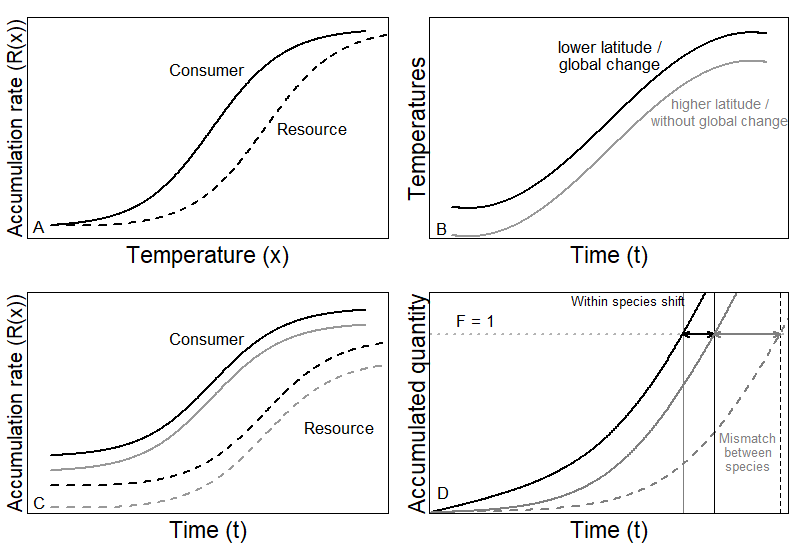
\includegraphics[width = 17 cm, keepaspectratio]{Conceptual}
    \caption{Illustration of theoretical development. Top left: The rate accumulation function for two different species (solid line is consumer and dashed line is resource). Top right: two simplified temperature time series (black line is warmer and grey line is cooler). Bottom left: Four combinations of rate accumulation; each species with two different temperature time series. Bottom right: The resulting end of the resting phase for the consumer in cooler (grey solid) and warmer (black solid) temperatures and for the resource in cooler temperatures (black dashed). The difference within species (grey vs black) indicates the shift in emergence in space (due to latitude or altitude) or time (due to global change). The difference between species (solid vs dashed) indicates the mismatch in the end of the seasonal resting phase for a fixed temperature regime (same location and same time).}
    \label{fig:generaltheory}
\end{figure}

\begin{figure}
    \centering
    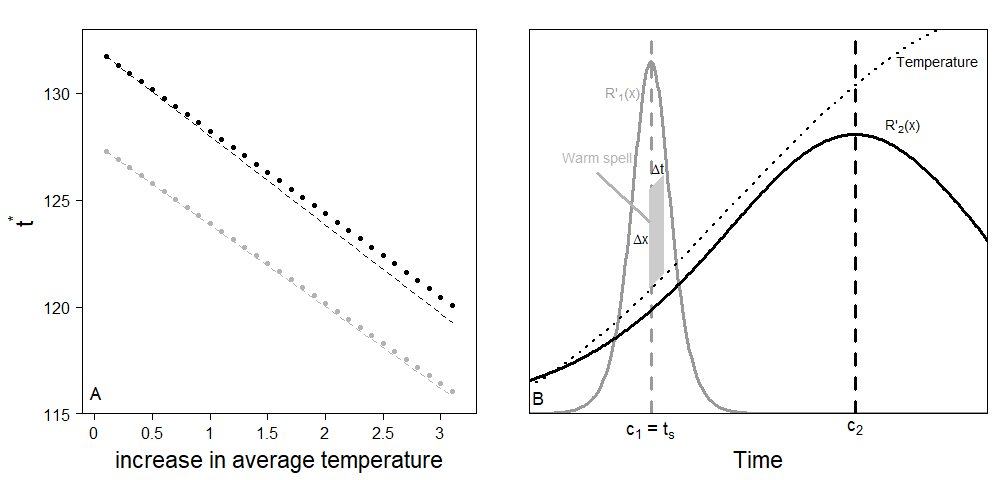
\includegraphics[width = 17 cm, keepaspectratio]{Figure2}
    \caption{Effects of (A) a constant temperature difference, and (B) a short warm spell, on species phenology. For both panels, black is the consumer (spruce budworm), and grey is the resource (balsam fir). (A) A constant temperature difference advances species phenology. Solid is the predicted value, dashed is the linear approximation from the model with simple time series. (B) The two species have their $R'$ that peaks at different temperatures. A short warm spell will mostly affect the species which $R'$ is highest at that time (in this example, the tree is more sensitive than the insect).}
    %\label{fig:my_label}
\end{figure}

\begin{figure}
    \centering
    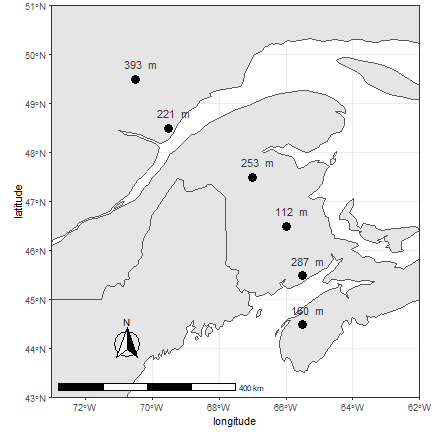
\includegraphics[width = 13 cm, keepaspectratio]{map_web}
    \caption{Location of the sample sites where temperature date were collected for past and future trends. Points are located across a gradient of latitude in Nova-Scotia, New Brunswick, and Quebec.}
    \label{fig:map}
\end{figure}

\begin{figure}
    \centering
    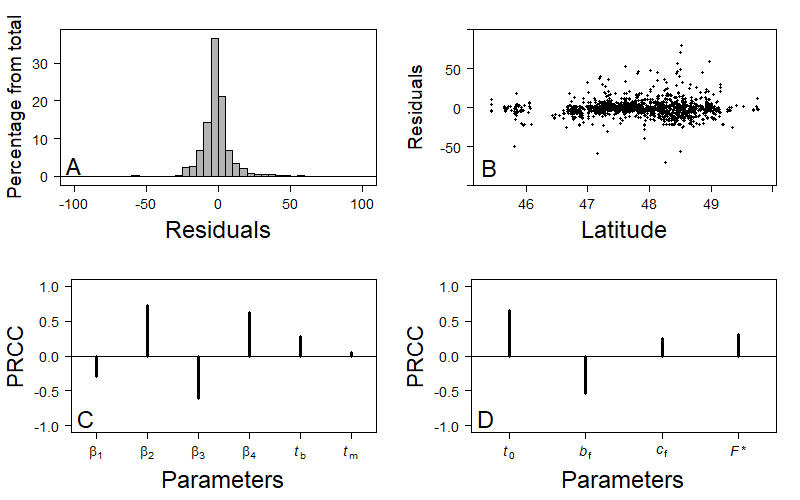
\includegraphics[width = 17 cm, keepaspectratio]{Sensitivity}
    \caption{Fitting residuals and sensitivity analysis of the Balsam fir model. (A) Residuals follow a Normal distribution centered on $0$. (B) No obvious latitudinal patterns can be found on the residuals within the range of latitudes that is used throughout the rest of the study. (C) Partial Rank Correlation Coefficient (PRCC) shows that the budworm model is sensitive to most parameters especially $\beta _2$, $\beta _4$ and $x_b$ that delay emergence, and $\beta _3$ that advance phenology. (D) The tree model is mostly sensitive to $b$ that advances budburst, and $t_1$ that delays budburst.}
    %\label{fig:my_label}
\end{figure}

\begin{figure}
    \centering
    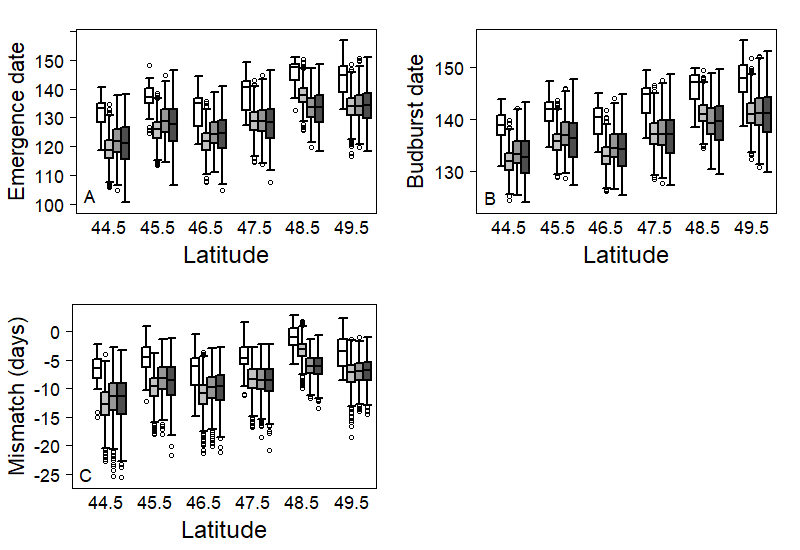
\includegraphics[width = 17 cm, keepaspectratio]{Total_Boxplots}
    \caption{Latitudinal distribution of (A) emergence date of $\text{L}_2$ instar (Julian days), (B) budburst date (Julian days), and (C) mismatch between emergence and budburst date. For each latitude, the white box (left one) represents the 1996-2016 period. Grey boxes represent expected outcome according to RCP $2.6$ (light grey), RCP $4.5$ (dark grey), and RCP $8.5$ (black) scenarios over 2021 to 2100.  Both emergence and budburst are expected to occur later at higher latitudes. Over all warming scenarios, both events are expected to occur earlier in the year. Warmer scenarios generate more variance. Nowadays, emergence is expected to occur 5 to 10 days before budburst at low latitudes, while at higher latitudes, emergence may sometimes occur before budburst and sometimes afterwards.  For all warming scenarios, an increase in mismatch is expected. At low latitudes, emergence may occur too early some years, which may lead to low survival of $\text{L}_2$. At higher latitudes, emergence is expected to systematically occur a few days before budburst, which would increase survival of $\text{L}_2$.}
    %\label{fig:my_label}
\end{figure}

\end{document}
